% !TEX option = -shell-escape
\documentclass[a4paper,12pt]{article}

%________________________  Langue et encodage ____________________
\usepackage[french,english]{babel} % Langue du document
\usepackage[T1]{fontenc} % Codage des caractères pour la gestion des accents
\usepackage[utf8]{inputenc} % Encodage UTF-8
\usepackage{paracol}
\usepackage{wasysym}

%____________________________ Mise en page _______________________ 
\usepackage[left=1.5cm,right=1.5cm,top=2cm,bottom=2cm]{geometry} % Gestion des marges
\usepackage{setspace} % Gestion des espaces interlignes
\usepackage{titlesec} % Personnalisation des titres de sections
\usepackage{titling} % Personnalisation du titre
\usepackage{fancyhdr} % Personnalisation des en-têtes et pieds de page
\usepackage{lastpage} 


%__________________________ Mathématiques ________________________
\usepackage{mathtools} % Paquet pour des équations et symboles mathématiques
\usepackage{siunitx} % Écriture avec la notation scientifique
\usepackage{pgfplots}

%________________________ Flottants et images ____________________
\usepackage[section]{placeins} % Forcer les flottants à rester dans les sections
\usepackage{graphicx} % Insérer des images
\usepackage[justification=centering]{caption} % Légendes centralisées
\usepackage{subcaption} % Sous-légendes pour des figures
\usepackage{wallpaper} % Utiliser des fonds ou des images de fond
\usepackage{wrapfig} % Mise en page personnalisée pour les images

%______________________________ Tableaux ___________________________
\usepackage{array,multirow,makecell} % Personnalisation avancée des tableaux
\usepackage{booktabs} % Amélioration des tables (lignes fines, moyennes, épaisses)
\usepackage{colortbl} % Coloration des cellules de tableaux
\usepackage{diagbox} % Pour créer des cellules en diagonale
\usepackage{longtable} % Tables sur plusieurs pages

%_____________________________ Code source _________________________
\usepackage{minted} % Mise en forme de code source avec coloration syntaxique
\usepackage{listings} % Insertion et mise en forme du code source

%______________________ graphie et références ______________________
\usepackage[backend=biber]{biblatex} % Gestion de la bibliographie
\addbibresource{./references.bib}

\usepackage{csquotes} % Gestion des guillemets typographiques
\usepackage[colorlinks=true, linkcolor=darkblue, urlcolor=darkblue]{hyperref}
\usepackage{cleveref} % Références intelligentes

% --- Textes et acronymes ---
\usepackage{acro} % Gestion des acronymes
\usepackage{nomencl} % Création d'une nomenclature (glossaire)
\makenomenclature % Commande pour générer la nomenclature

% --- Glossaires ---
\usepackage{glossaries}
\makeglossaries

\newcommand{\glossaryhref}[2]{\texorpdfstring{\href{#1}{\textcolor{black}{#2}}}{#2}}

% ----- Compteur pour les exposants glossaire ----------
\newcounter{glsref}
\renewcommand*{\theglsref}{\textsuperscript{\arabic{glsref}}}
% Sauvegarde de la commande originale 
\let\oldgls\gls
% Redéfinition de \gls pour ajouter l'exposant auto-incrémenté
\renewcommand{\gls}[1]{%
  \stepcounter{glsref}%
  \oldgls{#1}\theglsref%
}

% --- Dessins et graphiques ---
\usepackage{tikz} % Nécessaire pour smartdiagram
\usetikzlibrary{shapes.geometric, arrows.meta, calc, positioning}
\usepackage{eso-pic} % Gestion d'images en arrière-plan
\usepackage{tcolorbox} % Création de boîtes de couleur pour des équations ou du texte
\usepackage{smartdiagram} % Créer les figures simplement
\usesmartdiagramlibrary{additions} %Dépendances smartdiagram

% --- Divers ---
\usepackage{appendix} % Gérer les annexes
\usepackage{multicol} % Texte en colonnes
\usepackage{lastpage} % Référence à la dernière page
\usepackage{ragged2e} % Justification d'un texte à l'intérieur d'un parbox

\definecolor{darkpurple}{RGB}{102,0,153}
\definecolor{darkblue}{rgb}{0.0, 0.3, 0.6} % Bleu foncé pour les sections
\definecolor{darkgreen}{rgb}{0.0, 0.5, 0.0}  % Vert foncé
\definecolor{darkred}{rgb}{0.5, 0.0, 0.0}    % Rouge foncé
\definecolor{darkblack}{rgb}{0.1, 0.1, 0.1}  % Noir foncé (légèrement moins intense que le noir pur)
\definecolor{darkyellow}{RGB}{153,102,0}
\definecolor{darkgray}{RGB}{64,64,64}

% Formatage des sections
\titleformat{\section}[block]
  {\normalfont\Large\bfseries\rmfamily\color{darkblue}}  % Police, taille, graisse et couleur
  {\thesection}{1em}{}[\titlerule]                       % Numérotation et ligne sous le titre
\titlespacing{\section}{5pt}{10pt}{10pt}                 % Espacement avant et après
\renewcommand{\labelitemi}{\textemdash}

% Formatage des sous-sections
\titleformat{\subsection}[block]
  {\normalfont\large\bfseries\rmfamily\color{darkblue}}  % Police, taille, graisse et couleur
  {\thesubsection}{1em}{}                                % Numérotation
\titlespacing{\subsection}{5pt}{8pt}{5pt}                % Espacement avant et après

% Formatage des sous-sous-sections
\titleformat{\subsubsection}[block]
  {\normalfont\normalsize\bfseries\rmfamily\color{darkblue}} % Police, taille, graisse et couleur
  {\thesubsubsection}{1em}{} % Numérotation
\titlespacing{\subsubsection}{5pt}{8pt}{5pt} % Espacement avant et après

% Appliquer les liens en bleu et soulignés uniquement dans la bibliographie
\AtEndPreamble{\hypersetup{ colorlinks=true, linkcolor=black, urlcolor=darkblue,filecolor=black }}

% Redéfinir ma commande \bibliography pour personn
liser les liens
\usepackage{etoolbox}
\pretocmd{\bibliography}{ \hypersetup{ colorlinks=true,linkcolor=black, urlcolor=black, filecolor=black}}{}{}
\hypersetup{citecolor=darkblue,}

%---------------------------Diagramme de conclusion ----------------------------------------

% Définition de la mise en forme listing (pour l'intégration des codes et pseudoCode)
\definecolor{background}{HTML}{F1F1F0}
\definecolor{string}{HTML}{DD1144}
\definecolor{keyword}{HTML}{0077AA}
\definecolor{comment}{HTML}{44AA99}
\definecolor{identifier}{HTML}{000000}
\definecolor{framecolor}{HTML}{CCCCCC}

\lstset{
  backgroundcolor=\color{background}, % Couleur de fond
  basicstyle=\small\ttfamily, % Taille et police par défaut
  keywordstyle=\color{blue}, % Mots-clés en bleu
  commentstyle=\color{comment}, % Commentaires
  stringstyle=\color{string}, % Chaînes de caractères
  identifierstyle=\color{identifier}, % Identifiants
  numbers=left, % Numérotation des lignes
  numberstyle=\tiny\color{gray}, % Style de numérotation
  language=bash, % Langage utilisé (bash)
  frame=single, % Encadrement du code
  rulecolor=\color{framecolor}, % Couleur du cadre
  framesep=2pt, % Espacement autour du code
  framerule=0.5pt, % Épaisseur du cadre
  breaklines=true, % Retour à la ligne si le code est trop long
  morekeywords={grep, cut, tr, efetch, nano, build, touch, apptainer, run, shell}, % Ajouter && comme un mot-clé
  emph={\&\&}, % Emphases supplémentaires
  emphstyle=\color{red}, % Met en rouge les opérateurs &&
  inputencoding=utf8, % Encodage UTF-8 pour les caractères spéciaux
  extendedchars=true, % Permet l'utilisation des caractères spéciaux
  showstringspaces=false,
  literate=%
    {é}{{\'e}}1
    {è}{{\`e}}1
    {ê}{{\^e}}1
    {ë}{{\¨e}}1
    {à}{{\`a}}1
    {ç}{{\c{c}}}1
    {ù}{{\`u}}1
    {û}{{\^u}}1
    {î}{{\^i}}1
    {ï}{{\¨i}}1
    {ô}{{\^o}}1
}
\lstset{
  language=C++,                           % Langage utilisé
  basicstyle=\ttfamily\footnotesize,      % Police de base (taille et type)
  keywordstyle=\color{blue}\bfseries,      % Couleur et style des mots-clés
  commentstyle=\color{green!50!black},      % Couleur des commentaires
  stringstyle=\color{red},                  % Couleur des chaînes de caractères
  numbers=left,                           % Numérotation des lignes à gauche
  numberstyle=\tiny\color{gray},            % Style de la numérotation
  stepnumber=1,                           % Numérotation toutes les lignes
  numbersep=5pt,                          % Distance entre la numérotation et le code
  tabsize=4,                              % Taille des tabulations
  showspaces=false,                       % Ne pas afficher les espaces spéciaux
  showstringspaces=false,                 % Ne pas afficher les espaces dans les chaînes
  breaklines=true,                        % Retour à la ligne automatique
  breakatwhitespace=true,                 % Retour à la ligne uniquement aux espaces
  captionpos=b,                           % Position de la légende (b pour bottom)
  frame=single,                           % Encadrement du listing
  rulesepcolor=\color{gray}               % Couleur de la ligne d'encadrement
}
% Palette scientifique sobre
\definecolor{makefileText}{rgb}{0.12, 0.12, 0.12}             % Noir doux, plus élégant que pur noir
\definecolor{makefileBackground}{RGB}{245, 247, 250}          % Gris bleuté très clair
\definecolor{makefileKeyword}{rgb}{0.0, 0.28, 0.67}           % Bleu académique
\definecolor{makefileComment}{rgb}{0.0, 0.5, 0.0}             % Vert foncé, proche du LaTeX original
\definecolor{makefileString}{rgb}{0.55, 0.0, 0.0}             % Bordeaux sobre
\definecolor{makefileFrame}{gray}{0.65}                       % Gris neutre pour les bordures
\definecolor{makefileNumbers}{gray}{0.45}                     % Gris discret pour numéros de ligne

% Style Makefile haut niveau
\lstdefinestyle{makefileStyle}{
  language=sh,
  basicstyle=\ttfamily\footnotesize\color{makefileText},     % Police monospace et couleur douce
  backgroundcolor=\color{makefileBackground},                % Fond discret
  keywordstyle=\bfseries\color{makefileKeyword},             % Mots-clés bien visibles
  commentstyle=\itshape\color{makefileComment},              % Commentaires discrets mais lisibles
  stringstyle=\color{makefileString},                        % Chaînes de caractères bien différenciées
  frame=single,
  rulecolor=\color{makefileFrame},
  rulesepcolor=\color{makefileFrame},
  numbers=left,
  numberstyle=\tiny\color{makefileNumbers},
  numbersep=8pt,
  stepnumber=1,
  showstringspaces=false,
  breaklines=true,
  breakatwhitespace=true,
  columns=flexible,
  tabsize=2,
  xleftmargin=2em,
  xrightmargin=1em,
  aboveskip=1em,
  belowskip=1em,
  morekeywords={@mv,doxygen, for,done, fi, if, then, pdflatex, firefox, evince, mkdir, -p, @,mv, zcat, STAR, crac,gunzip, > , >> ,echo}     
}
% Définition du caption lstlisting
\renewcommand{\lstlistingname}{Code}

% Environnement spécifique pour Makefile
\lstnewenvironment{makefile}[1][]{
  \lstset{style=makefileStyle, #1}
}{}
%_________________________ Définition de la bibliographie ____________________
\title{Rapport DevOPS M1} %Titre du fichier

% Définir un nouvel environnement de flottant 
\newfloat{listing}{htbp}{lop}
\floatname{listing}{Code}
\newenvironment{lexique}{\begin{itemize}[itemsep=-5pt, left=0pt]}{\end{itemize}}

%__________Montage de la table des abbréviation___________

\setlength{\arrayrulewidth}{0.5mm}
\setlength{\tabcolsep}{10pt} % Ajuste l'espace entre les colonnes
\renewcommand{\arraystretch}{0.9} % Ajuste l'espacement des lignes

%-------------------------------------------------------------------------------------------------
%                              DEFINITIONS DU GLOSSAIRE 
%-------------------------------------------------------------------------------------------------
%________________________Définition de la mise en forme  des pieds de pages et en-tête ___________________
%Définir un fond d'image pour les pages sauf la première

\newcommand{\fairemarges}{
    \makenomenclature
    \pagestyle{fancy}
    \fancyhf{} % Réinitialise les en-têtes et pieds de page

    \setlength{\footskip}{-35pt} % Hauteur du pied de page
    \setlength{\headheight}{-10pt} % Hauteur de l'en-tête
    \setlength{\headsep}{0pt} % Espacement entre l'en-tête et le texte 
    % Contenu du pied de page
% Pied de page

\fancyfoot[L]{
    {\sffamily \Large \textbf{\thepage}} / \pageref{LastPage}
}

\fancyfoot[R]{
    {\sffamily \normalsize \textit{\nouppercase{\leftmark}}}
}  
    \renewcommand{\footrulewidth}{0.3pt} % Épaisseur de la ligne du pied de page
    \renewcommand{\headrulewidth}{0pt} % Épaisseur de la ligne de l'en-tête

    % Couleur des lignes
    \renewcommand{\footrule}{{\color{darkblue}\hrule width\headwidth height\footrulewidth \vskip-\footrulewidth}}
    \renewcommand{\headrule}{{\color{darkblue}\hrule width\headwidth height\headrulewidth \vskip-\headrulewidth}}
}

\fairemarges % Applique les marges et configurations

\onehalfspacing

\DeclareUnicodeCharacter{202F}{\,}

%-----------------------------Algorithmes -------------------------
\usepackage[linesnumbered, ruled, vlined]{algorithm2e}
\usepackage{algpseudocode}   % Pseudocode dans les algorithmes
\makeatletter
\algrenewcommand\ALG@beginalgorithmic{\normalfont\sffamily} 
\makeatother

% Définition des couleurs
\definecolor{bleumarine}{rgb}{0.0, 0.0, 0.5} % Bleu marine
\definecolor{rouge}{rgb}{0.8, 0.0, 0.0} % Rouge
\definecolor{fonction}{rgb}{0.0, 0.5, 0.4}
\definecolor{commentaire}{RGB}{100, 140, 100} 

% Personnalisation des mots-clés français
\SetKw{KwPour}{\hspace{-1cm}\sffamily \textcolor{bleumarine}{Pour}}
\SetKw{KwFinPour}{\hspace{-1cm}\sffamily \textcolor{bleumarine}{Fin Pour}}
\SetKw{KwSi}{\hspace{-1cm}\sffamily \textcolor{bleumarine}{Si}}
\SetKw{KwFinSi}{\hspace{-1cm}\sffamily \textcolor{bleumarine}{Fin Si}}
\SetKw{KwSinon}{\hspace{-1cm}\sffamily \textcolor{bleumarine}{Sinon}}
\SetKw{KwTantQue}{\hspace{-1cm}\sffamily \textcolor{bleumarine}{Tant Que}}
\SetKw{KwFinTantQue}{\hspace{-1cm}\sffamily \textcolor{bleumarine}{Fin Tant Que}}
\SetKw{KwRetourner}{\hspace{-1cm}\sffamily \textcolor{bleumarine}{Retourner}}
\SetKw{KwDebut}{\sffamily \textcolor{bleumarine}{Début}}
\SetKw{KwFin}{\sffamily \textcolor{bleumarine}{Fin}}
\SetKw{KwVariables}{\sffamily \textcolor{bleumarine}{Variables}}
\SetKw{KwFaire}{\sffamily \textcolor{bleumarine}{Faire :}}
\SetKw{KwAlors}{\sffamily \textcolor{bleumarine}{Alors :}}
\SetKw{KwEt}{\textcolor{bleumarine}{ ET }}
\SetKw{KwAfficher}{\hspace{-1cm}\sffamily \textcolor{bleumarine}{Afficher}}
\SetKw{KwFonction}{\hspace{-1cm}\sffamily {Fonction}}
\SetKw{KwOuvrir}{\hspace{-1cm}\sffamily {Ouvrir}}
\SetKw{KwTrier}{\hspace{-1cm}\sffamily \textcolor{bleumarine}{Trier}}
\SetKw{KwA}{\hspace{-1cm}\sffamily \textcolor{bleumarine}{A}}


% Configuration des numéros de ligne et indentations
\SetKwProg{Fn}{\vspace*{-2mm}\hspace{-5mm}}{}
\SetNlSty{}{} %Numéro de ligne
\SetAlgoNlRelativeSize{-1} % Ajustement des numéros de ligne

\newcommand{\CxCons}{\hspace{5mm}{\textcolor{gray}{O(1)}}} % constante
\newcommand{\CxLin}{\hspace{5mm}{\textcolor{gray}{O(n)}}} %linéaire
\newcommand{\CxQuad}{\hspace{5mm}{\textcolor{gray}{O(n^2)}}} % quadratique
\newcommand{\CxCub}{\hspace{5mm}{\textcolor{gray}{O(n^3)}}} % cubique
\newcommand{\CxPoly}{\hspace{5mm}{\textcolor{gray}{O(n^k)}}} % polynomiale
\newcommand{\CxExp}{\hspace{5mm}{\textcolor{gray}{O(2^n)}}} % exponentielle
\newcommand{\CxFact}{\hspace{5mm}{\textcolor{gray}{O(n!)}}} % factorielle
\newcommand{\CxLogLin}{\hspace{5mm}{\textcolor{gray}{O(n $\log$ n)}}} % n log

%_________________________ Montage du contour ____________________
\AtBeginShipout{
    \begin{tikzpicture}[remember picture, overlay]
        \draw [line width=0.1mm,gray!50!gray] 
            ($(current page.north west) + (0.5cm,-0.5cm)$) 
            rectangle 
            ($(current page.south east) + (-0.5cm,0.5cm)$);
    \end{tikzpicture}}
    

% Couleurs élégantes pour le code
\definecolor{bgcolor}{rgb}{0.95,0.95,0.95}   % Fond gris clair
\definecolor{commentcolor}{rgb}{0,0.5,0}      % Vert foncé pour les commentaires
\definecolor{keywordcolor}{rgb}{0,0,0.6}      % Bleu pour les mots-clés
\definecolor{stringcolor}{rgb}{0.6,0.2,0}     % Marron pour les chaînes
\definecolor{numbercolor}{rgb}{0.6,0,0}       % Rouge foncé pour les nombres

% Configuration avancée de listings
\lstdefinestyle{cppStyle}{
    language=C++,
    backgroundcolor=\color{bgcolor},
    basicstyle=\ttfamily\footnotesize,  % Police typewriter
    keywordstyle=\bfseries\color{keywordcolor},
    commentstyle=\itshape\color{commentcolor},
    stringstyle=\color{stringcolor},
    numberstyle=\tiny\color{numbercolor},
    numbers=left,
    numbersep=8pt,
    breaklines=true,
    breakatwhitespace=true,
    showstringspaces=false,
    frame=single,                        % Encadrement du code
    rulecolor=\color{black},              % Bordure noire
    captionpos=b,                         % Légende en bas
    tabsize=4,
    morekeywords={constexpr, nullptr, override, final},  % Ajout de mots-clés récents
    escapeinside={(*@}{@*)},               % Permet d'insérer du LaTeX dans le code
}
\renewcommand{\ttdefault}{pcr}  % Utilisation de Courier pour le code

\tikzstyle{commit} = [circle, minimum size=6mm, draw=blue!80, fill=blue!30, font=\footnotesize, text centered]
\tikzstyle{process} = [rectangle, rounded corners, minimum width=3cm, minimum height=1cm, text centered, draw=black, fill=orange!30]
\tikzstyle{arrow} = [thick,->,>=stealth]
% Configuration du style des captions
\captionsetup{
    labelfont={color=darkblue,bf}, % Met le label (ex. : "Figure") en bleu foncé et en gras
    font=small % Taille du texte des captions
}

\definecolor{processblue}{RGB}{102,153,204}   % doux bleu
\definecolor{techgray}{RGB}{169,169,169}      % gris pour les biais techniques
\definecolor{lightgray}{RGB}{240,240,240}     % fond léger
\definecolor{myborder}{RGB}{100,100,100}      % bordures sobres

\tikzstyle{startstop} = [ rectangle, rounded corners, minimum width=3cm, minimum height=1cm, text centered, draw=myborder, fill=lightgray, drop shadow]
\tikzstyle{process} = [rectangle, rounded corners, minimum width=3cm, minimum height=1cm,text centered, draw=myborder, fill=processblue!20, drop shadow]
\tikzstyle{techbias} = [rectangle, rounded corners, minimum width=3cm, minimum height=1cm, text centered, draw=myborder, fill=techgray!40, drop shadow]
\tikzstyle{arrow} = [thick,->,>=stealth]
\tikzstyle{smallbubble} = [ellipse,draw=blue!50!black,fill=blue!20,thick,align=center,minimum width=2.7cm,minimum height=1.2cm,text centered]
\tikzstyle{decision} = [diamond,draw=orange!80!black,fill=orange!20,thick,aspect=2.5,text centered,inner sep=1pt]
\tikzstyle{process} = [rectangle,draw=green!50!black,fill=green!20,thick,minimum width=2.5cm,minimum height=1cm,text centered]
\tikzstyle{formula} = [ rectangle,draw=purple!80!black,fill=purple!10,thick,text centered,rounded corners,minimum width=4.5cm,minimum height=0.9cm]

%---------------------------Diagramme de conclusion ----------------------------------------

% Styles spécifiques avec effet 3D simulé pour le schéma biais technique.
\tikzstyle{startstop2} = [nodebase, fill=red!30, draw=red!50, thick,,drop shadow]
\tikzstyle{process2} = [nodebase, fill=orange!30, draw=orange!50, thick, drop shadow]
\tikzstyle{techbias} = [nodebase, fill=green!30, draw=green!50, thick, drop shadow]
\tikzstyle{biobias} = [nodebase, fill=blue!30, draw=blue!50, thick, drop shadow]
\tikzstyle{highlightbox} = [rectangle, draw=blue!80, thick, rounded corners, minimum width=5cm, minimum height=1.5cm, drop shadow]

% Styles spécifiques avec effet 3D simulé pour l'organigramme normalisation
\tikzstyle{startstop} = [rectangle, rounded corners, minimum width=2.8cm, minimum height=1.2cm, text centered, draw=blue!40, thick, fill=blue!20, drop shadow]
\tikzstyle{process} = [rectangle, rounded corners, minimum width=3cm, minimum height=1cm, text centered, draw=orange!40, thick, fill=orange!20, drop shadow]
\tikzstyle{smallbubble} = [rectangle, rounded corners, minimum width=2.5cm, minimum height=1cm, text centered, draw=red!40, thick, fill=red!20, drop shadow]
\tikzstyle{decision} = [rectangle, rounded corners, minimum width=3cm, minimum height=1cm, text centered, draw=green!40, thick, fill=green!20, drop shadow]
\tikzstyle{formula} = [rectangle, rounded corners, minimum width=2.5cm, minimum height=0.8cm, text centered, draw=blue!30, thick, fill=blue!10, drop shadow]

\tikzstyle{arrow} = [
    ultra thick,       % Augmente l'épaisseur de la flèche
    ->,               % Pointe directionnelle
    >=Stealth,       % Style de pointe structuré (Triangle)
    draw=black!80,    % Couleur noire légèrement atténuée
    line cap=round,   % Extrémités des lignes arrondies pour un aspect lisse
    shorten >=1pt,    % Réduit l'espace avant la pointe
    shorten <=1pt     % Réduit l'espace après le trait
]

% Définition de "double copy shadow" pour effet 3D
\tikzset{
  double copy shadow/.style={
    preaction={
      draw=#1, line width=2pt, double distance=1pt, opacity=0.5
    },
  }
}
\tikzset{
        Avant/.style={
            rectangle, rounded corners=10pt,
            draw=green!700, fill=green!10, % Contours épais vert foncé et fond vert clair
            thick,
            minimum width=5.5cm, minimum height=2cm,
            text centered,
        },
        Inconv/.style={
            rectangle, rounded corners=10pt,
            draw=red!700, fill=red!10, % Contours épais rouge foncé et fond rouge clair
            thick,
            minimum width=5.5cm, minimum height=2cm,
            text centered,
        }
    }

 Homéostasie de l’ARN
L’homéostasie de l’ARN désigne l’ensemble des mécanismes qui régulent la production, la maturation, le transport et la dégradation des ARN pour maintenir un équilibre fonctionnel dans la cellule.

 Transport axonal
Le transport axonal permet le déplacement des organites, protéines et ARN le long de l’axone, assurant la communication et la survie neuronale sur de longues distances.

 Autophagie
L’autophagie est un processus cellulaire de recyclage qui dégrade et élimine les composants cellulaires endommagés, contribuant à l’homéostasie et à la protection contre le stress cellulaire.


\begin{document}

\printnomenclature

%___________________________ Montage de la page de garde ______________________________
\begin{titlepage}
% Bande large et claire en arrière-plan

% Image de fond avec réglage de l'opacité et de l'échelle
\begin{minipage}{0.35\textwidth}
\vspace{15mm}
    \centering
    
\includegraphics[height=2.5cm]{logo_FDS_rond.png} % Ajuste la hauteur
\vspace{5mm}
\end{minipage}
\begin{minipage}{0.3\textwidth}
\vspace{15mm}
    \centering
    
\includegraphics[height=2.5cm]{Logo_Bioinfo.png} % Ajuste la hauteur
    \vspace{5mm}
\end{minipage}
\begin{minipage}{0.3\textwidth}
    \vspace{15mm}
    \centering
    
\includegraphics[height=2.4cm]{Logo_UM.png} % Ajuste la hauteur
    \vspace{5mm}
\end{minipage}
\vspace{5mm}

% Cadre autour de la 
\begin{tikzpicture}[remember picture, overlay]
    \draw [line width=0.5mm] ($(current page.north west) + (1cm,-1cm)$) rectangle ($(current page.south east) + (-1cm,1cm)$);
\end{tikzpicture}

\centering % Centraliser le contenu
% Utilisation de minipage pour les logos

{\scshape\LARGE Master Bioinformatique \\ Université de Montpellier\par} % Nom de l'université
    \vspace{8mm}
{\scshape\Large HAU803I : Rapport de stage de M1  \par} % Sous-titre
\vspace{1cm}
\rule{\linewidth}{0.5 mm} \\[0.5 cm]
{\huge\bfseries Titre à choisir \par} \
\rule{\linewidth}{0.5 mm} \\[1.5 cm]

\begin{minipage}{0.5\textwidth} % Minipage pour faire deux colonnes
    \begin{flushleft} \large % Envoyer à gauche
    \emph{\textbf{Etudiant :}}\\ % Titre au-dessus des noms à gauche
    Mickael Coquerelle \\ % Remplacer pour chacun
    \end{flushleft}
\end{minipage}
~
\begin{minipage}{0.4\textwidth}
    \begin{flushright} \large
    \emph{\textbf{Professeur :}} \\
     Anthony Boureux \\
    \end{flushright}
\end{minipage}\\

\vspace{2cm}

\begin{quote}
    \itshape
\end{quote}
\vspace{1cm}
\begin{flushright}
    \itshape
\end{flushright}
\vspace{5mm}

\end{titlepage}

%---------------------------------------
% GENERATION DE L'ABSTRACT  
%--------------------------------------
\selectlanguage{french}
\begin{abstract}

a remplir
\newpage
\end{abstract}

%-------------------------------------------------------------------------------------------------
%                                    TABLE DES ABBREVIATIONS ET DES SYMBOLES
%-------------------------------------------------------------------------------------------------x
\setlength{\nomitemsep}{-2pt} % Réduit l'espacement entre les items de nomenclature
% Table des symboles
%\nomenclature{{\large \textbf{$R_e$}}}{Lectures alignés sur l'échantillon \(e\)}
%\nomenclature{{\large \textbf{$F_e$}}}{Fragments alignés pour l'échantillon \(e\)}
%\nomenclature{{\large \textbf{$L_g$}}}{Longueur du gène d'intérêt \(g\)}
%\nomenclature{{\large \textbf{$\lambda_{x}$}}}{Facteur d'échelle de l'élément x}
%\nomenclature{{\large \textbf{$M_{g,e}$}}}{M-value pour le gène \(g\) dans l'échantillon \(e\)}
%\nomenclature{{\large \textbf{$A_{g,e}$}}}{A-value pour le gène \(g\) dans l'échantillon \(e\)}
%\nomenclature{{\large \textbf{$w_{g,e}$}}}{Poids basé sur la variance des M-values pour le gène \(g\) dans l'échantillon \(e\)}
%\nomenclature{{\large \textbf{$NR_{x}$}}}{Lectures Normalisées de l'élément x }
%\nomenclature{{\large \textbf{$\Pi$}}}{Produit}
%\nomenclature{{\large \textbf{$\sum$}}}{Somme}
%\nomenclature{{\large \textbf{$M_{g}$}}}{Moyenne géométrique du gène \(g\)}
%\nomenclature{{\large \textbf{$Q3_{g}$}}}{Troisième quartile des valeurs d'expression du gène \(g\)}
%\nomenclature{{\large \textbf{$Med_{x}$}}}{Médiane de l'élément x}
%\nomenclature{{\large \textbf{$k$}}}{Référence}
\printnomenclature


\section*{Liste des abréviations}

\begin{paracol}{2} % Création de 2 colonnes
    % Première colonne : Liste des abréviations
    \begin{center}
    \textbf{Acronymes}
    \end{center}
\begin{tabbing}
    \hspace{2cm} \= \kill % Pour définir la première colonne
    \textbf{\textsc{ADN}} \> Acide DésoxyRiboNucléique \\
    \textbf{\textsc{DGE}} \> Analyse d'Expression Différentielle\\
    \textbf{\textsc{ARN}} \> Acide RiboNucléique \\
    \textbf{\textsc{API}} \> Application Programming Interface \\
    \textbf{\textsc{CVS}} \> Concurrent Versions System \\
    \textbf{\textsc{FP}} \> Faux Positifs \\
    \textbf{\textsc{FN}} \> Faux Négatifs \\
    \textbf{\textsc{KB}} \> KiloBase \\
    \textbf{\textsc{SLA}} \> Sclérose Latérale Amyotrophique \\
    \textbf{\textsc{RCS}} \> Révision Control System \\
    \textbf{\textsc{SHD}} \> Séquençage Haut Débit \\
    \textbf{\textsc{SNP}} \> Polymorphisme nucléotidique unique \\
    \textbf{\textsc{SIF}} \> Singularity Image Format \\
    \textbf{\textsc{UML}} \> Language de modélisation unifié\\
    \textbf{\textsc{VP}} \> Vrai Positifs \\
    \textbf{\textsc{VN}} \> Vrai Négatifs \\
 
\end{tabbing}
    \hspace{5mm}
    \switchcolumn % Passe à la deuxième colonne
    % Deuxième colonne : Liste des symboles mathématiques
\begin{center}
    \textbf{Symboles}
\end{center}
\begin{tabbing}
    \hspace{1.5cm}  \= \kill
    $\mathcal{A}_{\text{x}}$ \> Alphabet de x \\
    $\Sigma_{\text{x}}$ \> Somme de x \\
    $Q_{P}$ \> Score de qualité Phred\\
    $Q_{A}$ \> Score de qualité Phred encodé en ASCII\\
    $S$ \> Séquence biologique\\
    $P$ \> Motif recherché \\
    $S_e$ \> Sensibilité \\
    $S_p$ \> Spécificité\\
    $\mathcal{T}$ \> Texte \\
    $w$ \> Mot\\
    $\mathcal{O}()$ \> Notation de Landau\\
    $\mathcal{SA}_{x}$ \> Table des suffixes de x\\
\end{tabbing}

\end{paracol}


\addcontentsline{toc}{section}{Liste des abréviations et symboles}

%-------------------------------------------------------------------------------------------------
%                                    TABLE DES FIGURES, TABLEAUX ET CODES
%-------------------------------------------------------------------------------------------------
\selectlanguage{french}
%____________________  Montage de la table des figures et des tableaux _______________

% Définir un nouvel environnement de flottant pour minted
\newfloat{listing}{htbp}{lop}
\floatname{listing}{Code}

% Redéfinir le titre de la liste des listings
\renewcommand{\lstlistlistingname}{Liste des codes}
\newpage

%-------------------------------------------------------------------------------------------------
%                                            TABLE DES MATIERES
%-------------------------------------------------------------------------------------------------

\tableofcontents
\vspace{10mm}
\newpage

\section{Introduction}
%\begin{wrapfigure}{r}{0.5\textwidth} % Ajuste la largeur selon le besoin
 %   \vspace{-0.5cm} % Ajustement vertical
  %  \centering
   % \resizebox{0.5\textwidth}{!}{ % Réduire la taille
    %    \begin{tikzpicture}[scale=1, every node/.style={scale=0.9, anchor=east}]

	
    %}
   % \caption{\underline{Construction de $\mathcal{SA}_{T}$}}
   % \vspace{-0.5cm} % Ajuster l'espace sous la figure
%\end{wrapfigure}

\subsection{Environnement du stage}

Ce travail est la synthèse de mon stage de première année de Master, durant lequel j'ai intégré l'équipe de la professeure Thérèse Commes du laboratoire Bio2M,
 rattaché à l’Institut national de la santé et de la recherche médicale (INSERM). J'ai eu la chance d'être accompagné dans mon apprentissage par Anthony Boureux, enseignant-chercheur.
L'équipe est en collaboration étroite avec des services cliniques et des plateformes hospitalières, ce qui favorise évidemment l’innovation et la résolution de questions liées au champ médical.
Ainsi, j'ai eu l’occasion de contribuer à un projet de recherche translationnelle que Bio2M mène avec le CHU de Nîmes.  Ce travail est en lien direct avec des enjeux diagnostiques, puisqu’il concerne une maladie neurodégénérative : la sclérose latérale amyotrophique (SLA).
Les différentes missions qui m'ont étaient demandées s’inscrivent dans le champ de la transcriptomique, et tout particulièrement dans le cadre de l’analyse d’expression génique appliquée à la SLA, 
l’idée étant d’initier, proposé, une stratégie pour détecter une expression différentielle à l’échelle de certains gènes d’intérêt dans la SLA , avec des contraintes à la fois technique et biologiques,
 nous le verrons.

\subsection{Contexte biologique}

\begin{wrapfigure}{r}{0.50\textwidth} 
    \centering
    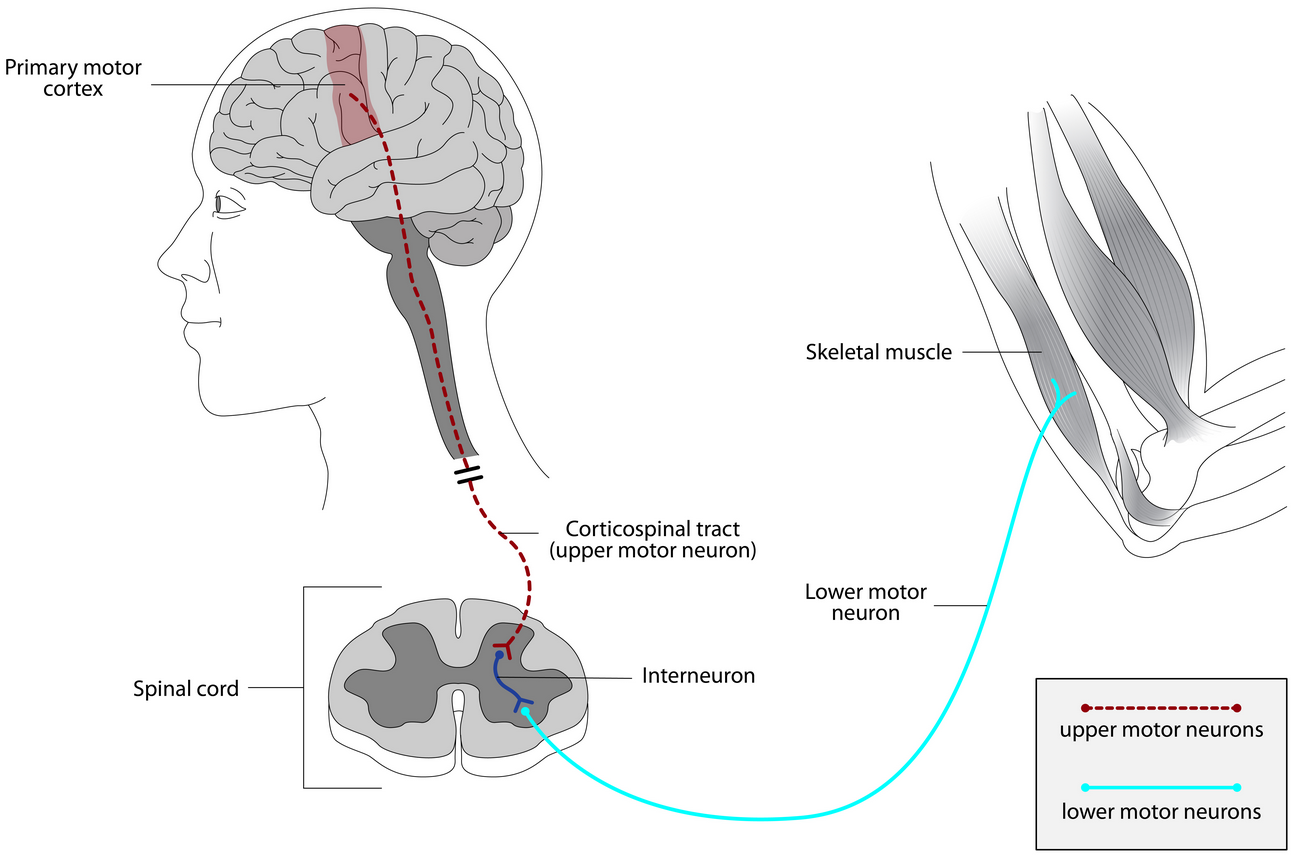
\includegraphics[width=1\linewidth]{Cortex_Spinal.jpg}
    \caption{\scriptsize{\textit{\underline{Atteinte neuronale dans la SLA(P.Wicks, 2024)}}}}
    \label{fig:Cortex}
\end{wrapfigure}

Une maladie rare se définit par une \hyperref[def:prevalence]{prévalence} de 0{,}05,\% dans la population générale.
 Quatre-vingts pour cent de ces maladies sont d’origine génétique~\textsuperscript{\cite{centre_constitutif_sla_de_tours_protocole_2020}},
 et la SLA en fait partie : elle touche un individu sur 20,000 en Europe~\textsuperscript{\cite{orphanet_prevalence_2023}},
  et sa prévalence mondiale varie de 1{,}57 à 11{,}8 pour 100,000 selon les pays, de l’Iran aux États-Unis~\textsuperscript{\cite{c_wolfson_et_al_global_2023}}.
C’est une maladie neurodégénérative causée par une atteinte du motoneurone central au niveau du cortex cérébral \textbf{(figure \ref{fig:Cortex})},
 et par une dégénérescence progressive des fonctions musculaires. Cette pathologie est très handicapante, tant sur le plan physique que social.
  En raison de sa gravité et des conséquences dévastatrices pour les patients et leur entourage, elle constitue un domaine de recherche de premier plan pour les généticiens. 
  C’est pourquoi il est pertinent d’intégrer une approche transcriptomique afin d’augmenter le rendement diagnostique des formes génétiques de la maladie et de mieux en comprendre les mécanismes.
Notons que les gènes responsables de la SLA sont globalement bien documentés. À ce jour, une quarantaine de gènes ont été identifiés et associés à la maladie. Dans 90\%
 des cas, leur implication est directe dans les formes familiales. Dans les 10\% restants, correspondant aux formes sporadiques, l’implication est plus indirecte, 
 via des perturbations de processus cellulaires clés tels que l’homéostasie de l’ARN, le transport axonal ou l’autophagie.
Enfin, on observe une forte hétérogénéité génétique, perceptible à travers l’implication de gènes aux fonctions parfois très différentes.,
 mais qui convergent toujours vers une dégénérescence neuronale. Les plus fréquemment impliqués sont  SOD1, TARDBP, FUS et C9ORF72~\textsuperscript{\cite{centre_constitutif_sla_de_tours_protocole_2020}},
  majoritaires dans la maladie ils constituent le socle des recherches génétiques pour tenter la mise au point de thérapies ciblées.

\subsection{Modéliser le signal biologique en données exploitables}

Supposons maintenant que l’on cherche à établir un profil d’expression génique pour notre quarantaine de gènes. 
Il faut alors s’interroger sur le support de lecture, c’est-à-dire le nombre de fois qu’une région d’ADN a été lue (ou comptée) au cours du séquençage.
On s'attend logiquement à avoir une densité de distribution de ces lectures, qui peut être intuitivement interprétée comme un reflet du niveau d’expression de chaque gène étudié.
En pratique, toutefois, un certain nombre de variables \textemdash ~ d’origine biologique ou expérimentale \textemdash ~ influencent cette expression théorique, introduisant une dispersion dans les données brutes.
A travers le schéma ci-dessous je présente un nombre non exhaustif de biais qui peuvent faussées l'expression génétique : 

\begin{figure}[ht]
    \centering
    \resizebox{0.8\textwidth}{!}{ 
    \begin{tikzpicture}[node distance=1.5cm and 1cm]

    \node (start) [startstop] {Prélèvement des échantillons : répétatibilité biologique ?};
    \node (step1) [process, below of=start, text width=6cm, align=center] {Extraction de l'ARN total};
    \node (step2) [process, below of=step1, text width=6cm, align=center] {Enrichissement de l'ARNm};
    \node (step3) [process, below of=step2, text width=6cm, align=center] {Fragmentation de l'ARN};
    \node (step4) [process, below of=step3, text width=6cm, align=center] {Synthèse de l'ADNc};
    \node (step5) [process, below of=step4, text width=6cm, align=center] {Préparation de la librairie};
    \node (step6) [process, below of=step5, text width=6cm, align=center] {Quantification de la librairie};
    \node (step7) [process, below of=step6, text width=6cm, align=center] {Séquençage};

    \node (note1) [techbias, right=3cm of step1, text width=6cm, align=center] {Pureté et Concentration extraite};
    \node (note2) [techbias, right=3cm of step2, text width=6cm, align=center] {Perte d'ARNm non poly-A};
    \node (note3) [techbias, right=3cm of step3, text width=6cm, align=center] {Fragmentation imparfaite};
    \node (note4) [techbias, right=3cm of step4, text width=6cm, align=center] {Efficacité reverse transcription};
    \node (note5) [techbias, right=3cm of step5, text width=6cm, align=center] {Thermocycleur, répétabilité};
    \node (note6) [techbias, right=3cm of step6, text width=6cm, align=center] {Variabilité de la quantification};
    \node (note7) [techbias, right=3cm of step7, text width=6cm, align=center] {Erreurs dues au séquençage};

    \draw [arrow] (start) -- (step1);
    \draw [arrow] (step1) -- (step2);
    \draw [arrow] (step2) -- (step3);
    \draw [arrow] (step3) -- (step4);
    \draw [arrow] (step4) -- (step5);
    \draw [arrow] (step5) -- (step6);
    \draw [arrow] (step6) -- (step7);

    \draw [arrow] (step1) -- (note1);
    \draw [arrow] (step2) -- (note2);
    \draw [arrow] (step3) -- (note3);
    \draw [arrow] (step4) -- (note4);
    \draw [arrow] (step5) -- (note5);
    \draw [arrow] (step6) -- (note6);
    \draw [arrow] (step7) -- (note7);

    %\node (note8) [biobias, right=0.5cm of step7, text width=2cm, align=center] {Illumina};
    %\node (note9) [biobias, right=0.2cm of step6, text width=2cm, align=center] {TapeStation};
    %\node (note10) [biobias, right=0.45cm of step5, text width=2cm, align=center] {Hamilton};
    %\node (note1) [biobias, right=0.5cm of step1, text width=2cm, align=center] {Nanodrop};

    % Ajout de la flèche verticale avec le texte "Processus"    
    \node[rectangle, rounded corners, draw=white, fill=gray!10, minimum width=10cm, minimum height=2cm, text width=2cm, align=center, anchor=north, rotate=90] at ([xshift=-5.4cm, yshift=-6cm]) {\textbf{Processus technique}};

    \end{tikzpicture}
    }
    \caption{\underline{\textit{ Schéma décisionnel pour normaliser les données RNASeq}}}
\end{figure}



\subsection{Etat de l'art}


\begin{figure}[ht]
\centering
\resizebox{1\textwidth}{!}{ 
\begin{tikzpicture}[node distance=1.5cm, every node/.style={font=\small}]

% ---------------------------------------------------
% Noeud de départ
\node (start) [smallbubble] {Quel objectif biologique ?};

% ---------------------------------------------------
% Questions initiales
\node (question1) [smallbubble, above left=1cm of start] {Comparaison globale ?};
\draw [arrow] (question1.south) |- (start.west);

\node (question2) [smallbubble, right=0.86cm of question1] {Analyse de gènes spécifique ?};
\draw [arrow] (question2.south) -- ++(0,0cm) -| (start.north);

\node (question3) [smallbubble, right=1cm of question2] {Quantification générale};
\draw [arrow] (question3.south) |- (start.east);

% ---------------------------------------------------
% Noeud de décision pour comparaison
\node (compare) [decision, below left=1.5cm of start] {Comparaison entre échantillons};
\draw [arrow] (start.south) |- (compare.east) node[midway, above, yshift=-1pt,xshift=-1.7cm] {\scriptsize{Soneson et al. 2016}};;

% ---------------------------------------------------
% Noeud de décision pour étude ciblée
\node (gene) [decision, below right=1.5cm of start] {Etude ciblée : un/des gènes};
\draw [arrow] (start.south) |- (gene.west) node[midway, above, yshift=-1pt,xshift=1.8cm] {\scriptsize{Zhao et al. 2021}};

% ---------------------------------------------------
% Méthodes de normalisation pour Comparaison
\node (TMM) [process, below=1.5cm of compare, xshift=-3cm] {TMM};
\node (RLE) [process, below=1.5cm of compare, xshift=2cm] {RLE};
\draw [arrow] (compare.south) -- ++(0,-1) -| (TMM.north);
\draw [arrow] (compare.south) -- ++(0,-1) -| (RLE.north);

% ---------------------------------------------------
% Références pour les méthodes de normalisation
\draw [arrow] (compare.south) -- ++(0,-1) -| (TMM.north) node[midway, right, yshift=6pt,xshift=-0.8cm] {\scriptsize{Robinson et al. 2010}};
\draw [arrow] (compare.south) -- ++(0,-1) -| (RLE.north) node[midway, right, yshift=6pt, xshift=-1.2cm] {\scriptsize{Anders et Huber 2010}};

% ---------------------------------------------------
% Formules sous les méthodes de normalisation
\node (TMMformula) [formula, below=2cm of TMM] {$TMM_{g,e} = \exp \left( \frac{\sum_{g} w_{g,e} M_{g,e}}{\sum_{g} w_{g,e}} \right)$};
\node (RLEformula) [formula, below=0.5cm of RLE] {$RLE_{ge} = \log_2\left(\frac{r_{ge}}{\text{Med}_g}\right)$};
\draw [arrow] (TMM.south) -- (TMMformula.north);
\draw [arrow] (RLE.south) -- (RLEformula.north);

% ---------------------------------------------------
% Méthodes de normalisation pour Quantification
\node (CPM) [process, below=1.5cm of gene,xshift=2cm] {CPM};
\node (FPKM_RPKM) [process, below left=1cm of CPM,xshift=-0.4cm] {FPKM \& RPKM};
\node (TPM) [process, below right=2cm and 0cm of CPM,minimum width=2cm] {TPM};

% ---------------------------------------------------
% Références pour les méthodes de quantification
\draw [arrow] (gene.south) -- ++(0,-1) -| (CPM.north) node[midway, right, yshift=6pt,xshift=-2cm] {\scriptsize{Anders et Huber 2010}};
\draw [arrow] (gene.south) -- ++(0,-1) -| (FPKM_RPKM.north) 
    node[midway, left, yshift=0.1cm, xshift=-0.3cm, rotate=90] {\scriptsize Mortazavi  2008}
    node[midway, right, yshift=-2.1cm, xshift=0.3cm, rotate=90] {\scriptsize{Derrien  2012}};

\draw [arrow] (gene.south) -- ++(0,-1) -| (TPM.north) node[midway, right, yshift=6pt,xshift=0.3cm,rotate=270] {\scriptsize{Parker et al. 2016}};

% ---------------------------------------------------
% Formules pour Quantification
\node (CPMformula) [formula, below=0.5cm of CPM] {$\displaystyle CPM_{g,e} = \frac{R_g}{\frac{\sum{r_e}}{\lambda}}$};
\node (FPKM_RPKMformula) [formula, below=1cm of FPKM_RPKM] {$\displaystyle FPKM_{g,e} = \lambda \times \frac{F_g}{L_g \times \sum_{e}F_e} $};
\node (TPMformula) [formula, below=1.5cm of TPM,xshift=0cm] {$TPM_{g,e} = \lambda \times \frac{{RPK}_{g,e}}{\sum_{e} \left(\frac{R_e}{L_e}\right)}$};

% Relier les flèches aux formules
\draw [arrow] (CPM.south) -- (CPMformula.north);
\draw [arrow] (FPKM_RPKM.south) -- (FPKM_RPKMformula.north);
\draw [arrow] (TPM.south) -- (TPMformula.north);

% ---------------------------------------------------
% Loi binomiale négative
\node (negBinom) [process, below=1.5cm of {$(RLEformula)!1!(TMMformula)$}] {Loi binomiale négative};
\draw [arrow] (negBinom.south) -- ++(0,-1);
% Relier les flèches des formules à la loi binomiale négative
\draw [arrow] (RLEformula.south) -- (negBinom.north) node[midway, above, yshift=-5pt, xshift=1.5cm] {\scriptsize{Duncan et al. 2009}}; 


% ---------------------------------------------------
% Formule de la loi binomiale négative
\node (LBNformula) [formula, below=1cm of negBinom] {$P(C_{g,e} = k) = \binom{r+k-1}{k} p^r (1-p)^k$};

% Relier la LBN à sa formule
\draw [arrow] (negBinom.south) -- (LBNformula.north); 

\end{tikzpicture}
}
\caption{\underline{\textit{ Schéma décisionnel pour normaliser les données RNASeq}}}
\end{figure}

 doivent elles être intégrées à l'analyse finale ? Cette question vas être pertinente dans une étude quantitative comme ici, puisqu'il s'agit, en autre, de caractériser une eventuelle haplo-insuffisance ou surexpression. 
 Nous allons comparer les différentes stratégies.Le périmètre de ce travail préliminaire était de faire un état des lieux des méthodes conventionnelles de normalisation,
pour \textit{in fine} détecter une éventuelle expression génétique différentielle à partir des données issues du séquençage RNA-Seq.
En effet, la transcription, étant fondatrice de la diversité protéomique, est par nature source de nombreuses anomalies génétiques. À l’issue de ce mécanisme,
un gène peut exprimer plusieurs isoformes dont l’impact peut être pathologique. Identifier de telles anomalies implique la création d’un protocole de séquençage spécifique et
d’un pipeline d’analyse RNA-Seq. L’objectif, à terme, est de déployer ce \textit{workflow} en intégrant une dimension transcriptomique pour le diagnostique de la SLA.\\
Durant mon premier semestre, j’ai eu l’occasion d’effectuer un travail de recherche bibliographique pour étayer ma compréhension des différentes approches permettant de mettre en œuvre cette étape.
La synthèse de ce travail préliminaire peut s’apprécier à travers la figure de synthèse ci-dessous :



Après avoir explorer les différentes méthodes de normalisation, en mettant particulièrement l'accent sur TMM, RLE et LBN, qui apportent une valeur ajoutée dans le contexte du RNA-Seq ciblé. Cette analyse repose sur plusieurs critères de performance clés en génétique, tels que les comparaisons inter-individuelles et la robustesse face aux valeurs extrêmes.
 L'objectif final etait d'évaluer l'approche la plus adaptée  d'un panel de gènes ciblés .

\subsection{Performance à faible profondeur et robustesse aux valeurs extrêmes} \vspace{3mm} Un des principaux critères d’évaluation est la robustesse aux valeurs extrêmes. Lorsqu’on cherche à établir un profil d'expression pour une maladie rare, comme la SLA, il est essentiel de déterminer si les valeurs de comptage aux extrémités de la distribution doivent être intégrées à l'analyse finale. Cette question peut être pertinente dans une étude quantitative visant à caractériser une éventuelle haplo-insuffisance ou surexpression. Nous allons comparer les différentes stratégies.\\

Les méthodes dites \textit{"Total Count"}, comme CPM, bien qu’utilisées pour leur simplicité, sont particulièrement sensibles aux valeurs extrêmes\textsuperscript{\cite{dillies_comprehensive_2013}}. Elles considèrent peu d'informations et ne permettent pas une évaluation efficace de la dispersion des données. Dans un contexte où l'expression génétique varie, elles se révèlent inadéquates. De même, FPKM et TPM présentent des limitations similaires. Ces méthodes sont souvent critiquées pour leur manque de reproductibilité et leur rigueur scientifique. Par exemple, \citeauthor{robinson_scaling_2010} (2010) ont montré que la division par la longueur du gène amplifie l’effet des valeurs aberrantes, surtout pour les gènes courts ou faiblement exprimés\textsuperscript{\cite{anders_differential_2010}}. Les travaux de \citeauthor{zhao_tpm_2021} (2021) confirment également cette limite. Quant à la méthode "Upper Quartile", cela est plus nuancé, car elle élimine les données du quartile inférieur\textsuperscript{\cite{dillies_comprehensive_2013}}, donc partiellement les valeurs extrêmes, mais elle reste peu adaptée à notre contexte où certains gènes peuvent être faiblement ou fortement exprimés par rapport à ce qui est attendu biologiquement.\\

A l'inverse, TMM, qui prend en compte la composition de l’ARN au moment de la normalisation, offre une meilleure résistance aux biais causés par les valeurs extrêmes\textsuperscript{\cite{robinson_scaling_2010}}. C'est aussi le cas pour RLE, grâce à l’utilisation de la médiane comme paramètre de position, qui donne une tendance centrale. Enfin, LBN repose sur l’hypothèse que les gènes ne sont pas différentiellement exprimés entre les conditions, ce qui renforce sa pertinence pour analyser les extrémités de la distribution. Ces trois approches partagent une philosophie commune : estimer le facteur de normalisation à partir d’un ensemble de gènes supposés stables.

\subsection{Compromis entre facilité d'interprétation et la pertinence biologique}

Après avoir fait un panorama des différentes stratégies mathématiques pour traiter les comptages bruts, il est évident que la diversité des méthodes peut paraître déroutante. Finalement, ce qui va être essentiel pour le biologiste, c'est de lui proposer une approche qui repose sur un compromis entre facilité d'interprétation et pertinence médicale. Le biologiste doit être en mesure de comprendre les corrections pour les relier aux décisions diagnostiques. Les méthodes conceptuellement simples comme CPM et UQ sont éliminées des options disponibles pour le périmètre de notre étude, car nous avons montré que, avec des échantillons présentant des variations biologiques importantes, la normalisation conduira à des conclusions erronées. Nous avons vu que les métriques comme TPM et FPKM sont des approches moins avancées que TMM, RLE et LBN, qui sont également plus simples à comprendre et à implémenter que les autres, mais elles manquent de correction statistique pour les comparaisons inter-échantillons.\\

En conclusion, la piste à creuser dans le périmètre de notre étude pencherait vers TMM ou RLE, et venir modéliser avec la LBN la surdispersion. Dans la littérature, il est régulièrement fait référence que la solution adéquate réside dans l'application d'une double correction\textsuperscript{\cite{robinson_scaling_2010}}. Comme nous l'avons souligné dans la méthodologie de la LBN, une fois que les biais techniques sont absorbés (par la correction RLE ou TMM), la méthode LBN peut être appliquée pour l'analyse de l'expression différentielle. Cette stratégie répondra à la fois à la problématique de la surdispersion et permettra d'obtenir une estimation précise de la variabilité inter-individuelle. Enfin, il est intéressant de mentionner que la taille de l'échantillon statistique (nombre de librairies) est directement corrélée à la puissance de la correction LBN. Comme souvent en statistique : plus les données seront consistantes plus la correction le sera également. Une piste de travail pour s'adapter aux contraintes de temps et de coût au laboratoire et pouvoir appliquer de manière crédible ces corrections serait donc de compiler (TMM ou RLE avec LBN) les données des diagnostics des librairies successives, semaine après semaine, pour augmenter la taille des données.
 Bien évidemment, cela doit se faire sous contrôle d'analyses statistiques pour valider une telle approche. 
C'est une option à envisager pour fournir un modèle probabiliste puissant pour l'analyse d'expression malgrès les contraintes organisationnelles (8 échantillons par expérience).


 doit être apprécié en considérant que chaque méthode a ses avantages et inconvénients, et le choix sera fait sur un certain nombre de critères,
  en tenant compte des spécificités des données et de l'objectif(s) biologique(s). Ce sujet sur la normalisation des données RNA-Seq dans le cadre du panel de gènes ciblés
   nous a permis de mettre en lumière la complexité de cette étape de normalisation des données RNA-Seq et la nécessité d'une collaboration étroite entre biologistes et bioinformaticiens 
   pour faire parler efficacement les résultats expérimentaux 


\subsection{Le problème}

Avant tout, rappelons que nous travaillons sur une maladie constitutionnelle. Par conséquent, il y a une très faible probabilité d'analyser des échantillons distincts pour un même patient à un intervalle de temps raisonnable, ce qui a peu de sens d'un point de vue de la génétique constitutionnelle, sauf dans des cas particuliers comme les études familiales. La notion de variabilité intra-individuelle est une qualité à étudier sur une matrice biologique identique. De manière générale, au laboratoire de génétique, il s'agit du sang, dans un milieu de transport adapté (tube STRECK pour l'ARN). Si ces conditions ne sont pas respectées, cela pourrait plutôt refléter une hétérogénéité biologique inhérente à une régulation de l'expression liée à la nature même du tissu, aux conditions de transport, à la variabilité de l'environnement analytique, avant même de songer à absorber les différents biais.
Il est donc fondamental d'avoir une planification expérimentale aussi standardisée que possible et d'un référencement complet et précis des biais biologiques connus et d'en évaluer leur impact.
Évaluer les biais biologiques et techniques est délicat. Comme nous l'avons vu plus haut, ils peuvent être confondus (préparation de la librairie, effets de lots, longueur des gènes, etc.).
La littérature aborde cet aspect sous des angles parfois différents, et les conclusions sont attribuées à des facteurs techniques et/ou biologiques, car il est difficile de faire la distinction. 
 Chaque expérience étant unique, chaque prélèvement l'est aussi, notamment par ses délais et ses modalités d'acheminement. Pour capturer au mieux ces sources de variabilité, et à travers les différentes études comparatives, 
 j'ai constaté que les méthodes les méthodes conventionnelles présentées en \textbf{figure 1} ne sont pas ou peu adapté au RNASeq ciblé pour faire de DGE. Ceci s'explique par leurs modalités de calcul, qui intègrent la dispersion et la comparaison inter-échantillons à l'échelle du transcriptome ~\textsuperscript{\cite{dillies_comprehensive_2013}}. TMM, en utilisant une moyenne tronquée des ratios de lectures pour calculer les facteurs de normalisation,
  va corriger efficacement les biais liés à la taille de la librairie (profondeur de séquençage notamment) et à la composition de l'ARN (régions riches en GC)\textsuperscript{\cite{abrams_protocol_2019}}.
 
    Présentation du jeu de données : 72 échantillons de transcriptomique ciblée (56 gènes SLA).
    Organisation en runs de séquençage (n = 8 par run).
    Limites méthodologique,  absence de gènes de référence stables, peu de données pour une normalisation robuste.
    Constats initiaux : forte variabilité de profondeur de lecture inter-run, faible reproductibilité.

\section{Matériels \& Méthodes}
\subsection{Génération des fichiers d’alignement}
    Stratégie de génération automatisée des fichiers BAM à partir des paires FASTQ (1 \& 2).
    
    Structure de traitement par run (batch de 8 échantillons).

    Mise en place d’un pipeline reproductible.
\subsection{Analyse de la variabilité expérimentale}

    Statistiques descriptives sur la profondeur de lecture, par run et par échantillon.

    Mise en évidence de la non-reproductibilité : inter-run vs. intra-run.

    Visualisations pour illustrer la disparité de couverture.

\subsection{Alignement : levée d’ambiguïté sur la variabilité}

    Présentation de STAR et CRAC :

        Méthodologie, hypothèses sous-jacentes, différences de traitement.

    Alignement des mêmes échantillons avec les deux outils.

    Comparaison des métriques de mapping : taux d’alignement unique/multiple/non-aligné.

    Conclusion : validation que l’étape d’alignement n’est pas responsable de la variabilité observée.

\subsection{Vers une approche alternative de quantification}

    Justification du besoin de s’affranchir des biais d’alignement.

    Introduction à la quantification par k-mer : promesse de neutralité méthodologique.

    Transition vers une stratégie plus robuste de détection différentielle.

\subsubsection{Qualité et spécificité de l'alignement}

L'étape de \og \textit{mapping} \fg dans un processus d'analyse est une étape charnière et pour notre cas d'étude on peut raisonnablement penser que cette étape peut biaiser le signal biologique réel, 

Pour évaluer si les deux outils d’alignement, STAR et CRAC, diffèrent significativement dans leur capacité à aligner les lectures uniques,
 j’ai réalisé une analyse statistique sur les proportions relatives des lectures uniques par patient.J’ai d’abord effectué un test de normalité de Shapiro-Wilk sur les données 
 de proportions de lectures uniques pour chaque outil afin de vérifier l’hypothèse de normalité nécessaire pour utiliser un test paramétrique. 
 Les résultats ont validé cette hypothèse, j’ai donc pu appliquer un test t de Student apparié pour comparer les moyennes des proportions de lectures uniques entre STAR et CRAC. 
 Le test t n’a pas montré de différence statistiquement significative (p > 0.05) entre les deux outils, ce qui suggère que, globalement,
  leur capacité à aligner des lectures uniques est comparable dans mon jeu de données.

Cependant, je tiens à souligner que ces résultats quantitatifs ne reflètent pas nécessairement les différences qualitatives dans les approches d’alignement de STAR et CRAC.
 En effet, ces deux outils reposent sur des algorithmes différents, avec des stratégies distinctes pour gérer les lectures multiples, les lectures chimériques, et les jonctions d’épissage. 
 Ces différences peuvent influencer la localisation précise des alignements, la sensibilité à certains types de variants, ainsi que la qualité globale des données alignées.
Par conséquent, même si la proportion de lectures uniques est comparable, j’interprète ces résultats avec prudence. Pour les analyses de quantification ultérieures,
 je recommande d’intégrer une étude plus approfondie des alignements, incluant une inspection visuelle des lectures alignées et une analyse des différences dans les catégories de lectures multiples 
 et chimériques. Cela me permettra de m’assurer que la variabilité introduite par les différences d’algorithmes n’impacte pas les conclusions biologiques que je tirerai des données.

\section{Résultats & discussion}
\subsection{Analyse de la variabilité expérimental et levée d'ambiguité sur l'alignement}
 
Il est intéressant de vérifier  si les deux outils d’alignement diffèrent significativement dans  
leur capacité à aligner de manière unique les lectures. Dans un premier temps j'ai construit à partir de mon fichier tabulé issue du script Bash  Pour ce faire, j’ai réalisé une analyse statistique sur les proportions relatives des lectures uniques par patient.  
J’ai commencé par effectuer un test de normalité de Shapiro-Wilk~\textsuperscript{\cite{shapiro_wilk_1965}} sur les données de proportions de lectures uniques pour chaque outil,  
afin de vérifier l’hypothèse de normalité nécessaire à l’utilisation d’un test paramétrique.~\textsuperscript{\cite{statistical_test_2021}}

Les résultats du test ne m’ont permis de rejeté cette hypothèse ; j’ai donc opté pour une approche non paramétrique plus robuste : le test de Wilcoxon ~\textsuperscript{\cite{wilcoxon_signed_rank_1945}} pour échantillons appariés.  

Il permet de comparer les distributions des proportions de lectures uniques entre \texttt{STAR} et \texttt{CRAC}, tout en tenant compte de la structure appariée des données (chaque patient servant de contrôle pour lui-même en quelque sorte).

Mon objectif est ici de déterminer si les différences observées dans les taux d’alignement unique relèvent de fluctuations aléatoires ou d’une divergence systématique entre les deux méthodes d’alignement. Pour autant il ne s'agit pas d'une comparaison d'outil en bon et due forme, mais de regarder grossièrement dans qu'elle mesure deux stratégies différentes pourraient influer sur la profondeur de lectures alignés. Subsidiairement, si il existe une significativité, est ce que cela peut influer en tout ou partie sur la variabilité des unités de comptages (nombres de lectures alignés à une position). 

\begin{figure}[H]
\begin{flushleft}
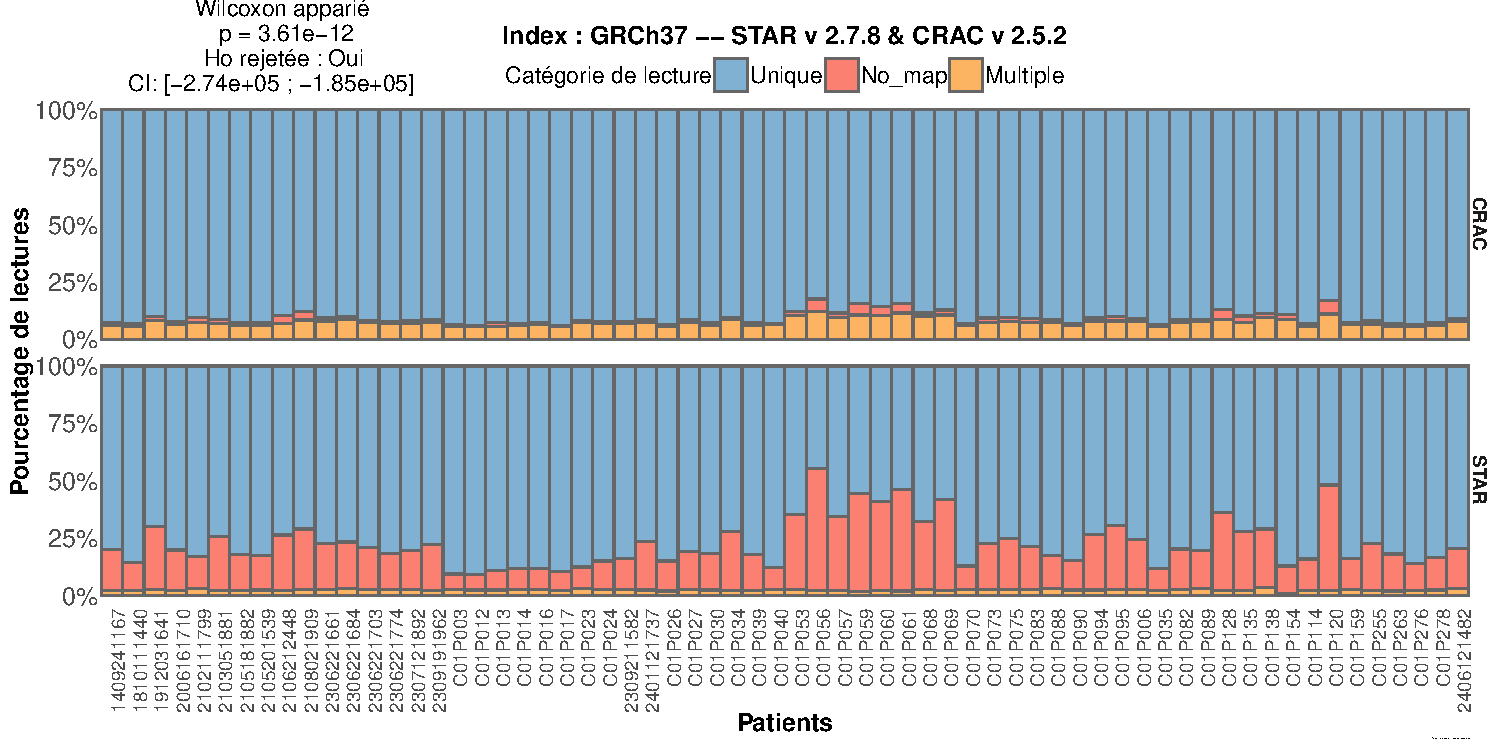
\includegraphics[width=1\linewidth]{Figure_STAR_CRAC_P.pdf}
\caption{\underline{Comparaison des profils d'alignement par patient entre STAR et CRAC}}
\label{fig:mappingp}
\end{flushleft}
\end{figure}

Soulignons ces résultats ne reflètent pas nécessairement une différence de qualité dans l’alignement entre \texttt{STAR} et \texttt{CRAC}. Comme évoqué précédemment, les stratégies algorithmiques diffèrent, notamment dans la manière de classifier les lectures uniques, multiples, et enfin celles non mappées. Ces divergences peuvent influencer la sensibilité de détection à certains types de variants.

\begin{figure}[H]
\begin{center}
\resizebox{1.05\textwidth}{!}{  
    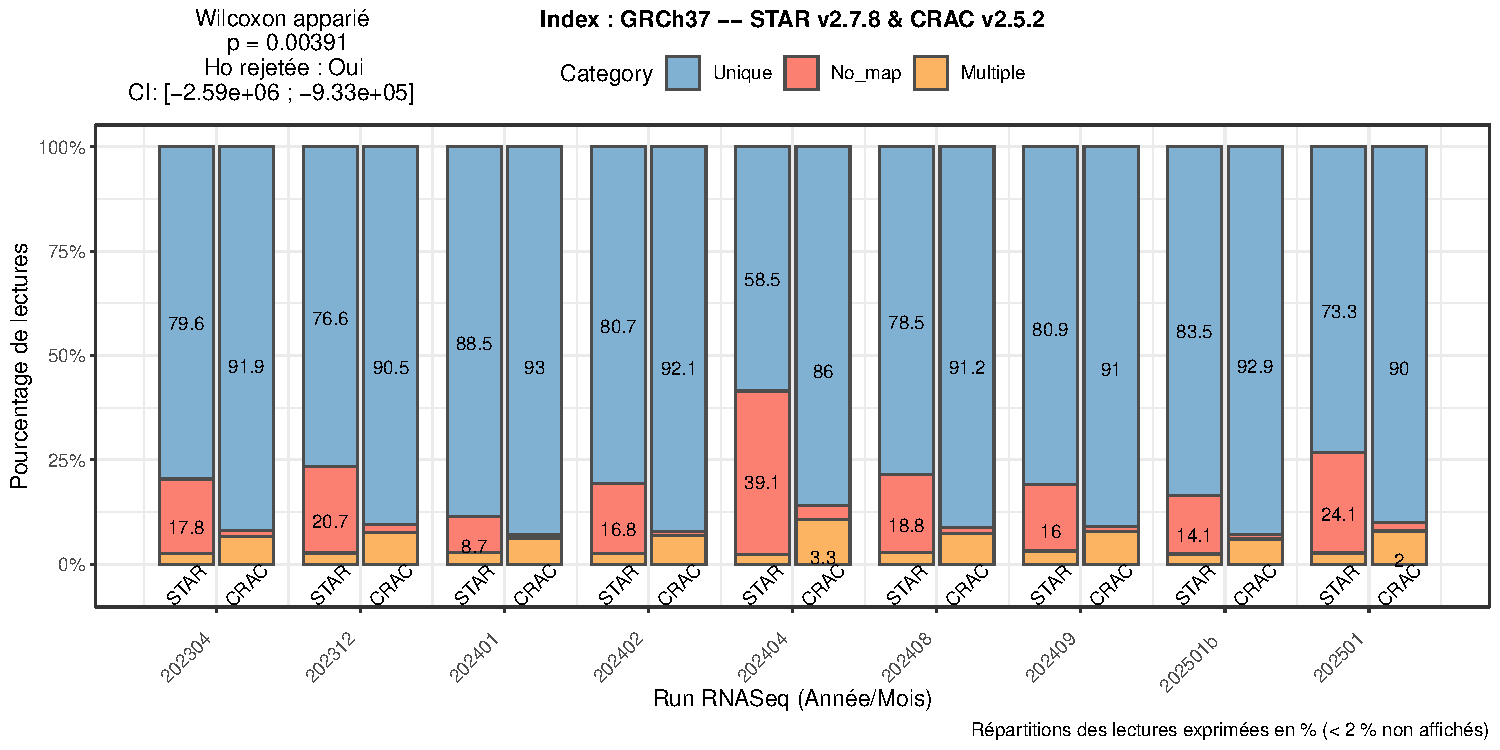
\includegraphics[width=1\linewidth]{Figure_STAR_CRAC_R.pdf}}
    \caption{\underline{Profils d'alignements par run entre STAR et CRAC}}
    \label{fig:mappingr}
\end{center}
\end{figure}

L'analyse statistique par test de Wilcoxon apparié révèle une différence significative entre le nombre de lectures uniques alignées par STAR et CRAC (\( p = 0{,}00391 \)). L'intervalle de confiance négatif \([-2{,}59 \times 10^{6} ; -9{,}33 \times 10^{5}]\) nous indique que \texttt{CRAC} (dans le paramétrage par défaut et pour notre cas d'étude précis) génère de manière systématique un nombre de lectures alignées de manière unique significativement plus élevé que \texttt{STAR} pour un même échantillon. Ce résultat suggère soit une sensibilité accrue, soit une stratégie d’alignement plus permissive. Par conséquent, même si la proportion de lectures uniques est  globalement comparable entre les deux outils (conclusion que l'on peut admettre autant à l'échelle du patient (\textbf{figure \ref{fig:mappingp}}) qu'a l'échelle du \textit{run} RNASeq \textbf{figure \ref{fig:mappingr}}. Avant d'éffectuer des analyses de quantification, j’ai mené des explorations complémentaires en extrayant la métrique nommée \og NH \fg (\textit{Number of Hits}), cette information est un champ dans le fichier de sortie au format \texttt{SAM}. Pour ce faire, j’ai développé un script Bash (cf. \textbf{Annexe à ajouter}). L'intérêt ici est d'essayer de comprendre la différence de lectures uniques entre les deux outils. 



    Statistiques descriptives sur la profondeur de lecture, par run et par échantillon.
    Mise en évidence de la non-reproductibilité : inter-run vs. intra-run.
    Visualisations pour illustrer la disparité de couverture.

    Présentation de STAR et CRAC :
    Méthodologie, hypothèses sous-jacentes, différences de traitement.

    Alignement des mêmes échantillons avec les deux outils.

    Comparaison des métriques de mapping : taux d’alignement unique/multiple/non-aligné.

    Conclusion : validation que l’étape d’alignement n’est pas responsable de la variabilité observée.


\subsection{Analyse des données de comptages avec normalisation TPM}



\subsection{Analyse des données de comptages avec normalisation TMM}

    Le test évalue si, pour un gène donné, l’expression normalisée (CPM\_TMM) est stitistiquement différente entre les conditions (ex: patients vs contrôles).
    Une p-value faible (<0.05 généralement) indique que la différence observée est peu probable due au hasard, donc potentiellement biologiquement significative.
    Ce test est robuste face aux distributions non normales, ce qui est fréquent en RNA-seq.
    Cependant, ce test ne donne pas d’indication sur la taille de l’effet (seulement s’il y a une différence significative).
    Sur 56 tests (un par gène), il faut ajuster la p-value pour réduire les faux positifs.
    
Modalités de calcul du test Wilcoxon (Mann-Whitney)
    Classe toutes les valeurs des deux groupes combinés (conditions) par ordre croissant.
    Attribue un rang à chaque valeur.
    Calcule la somme des rangs pour un groupe.
    Compare cette somme avec la distribution attendue si les deux groupes venaient de la même population.
    La p-value correspond à la probabilité d’obtenir une somme de rangs aussi extrême (ou plus) sous l’hypothèse nulle (pas de différence entre conditions).
Graphique
 j'affiche la distribution des CPM normalisés par gène, par condition, avec des points colorés.
    L’annotation avec label permet d’afficher la p-value pour chaque gène, informant visuellement sur la significativité des différences observées.
    Cela m’aide à relier visuellement l’intensité d’expression avec la signification statistique.
    
L’absence de différences statistiquement significatives (p > 0.05) dans les niveaux d’expression normalisés (CPM TMM) des 56 gènes d’intérêt entre les conditions étudiées suggère que, au sein des échantillons analysés, ces gènes ne présentent pas de variations d’expression marquées ou robustes en lien avec le facteur expérimental considéré. Cela peut indiquer que, dans ce contexte biologique précis, la modulation transcriptionnelle de ces gènes n’est pas significativement impactée par la condition testée, ou que les effets sont trop faibles pour être détectés avec la taille d’échantillon actuelle. Il est aussi possible que la variabilité inter-individuelle ou technique masque de potentielles différences subtiles. Enfin, ces résultats invitent à considérer d’autres niveaux de régulation (post-transcriptionnel, épigénétique) ou des approches complémentaires (ex. analyses multi-omics, échantillonnages plus larges) pour mieux comprendre les mécanismes biologiques sous-jacents dans cette pathologie ciblée.

   
    


\newpage
\section{Annexes}
\subsection{Structures des fichiers de log pour \texttt{STAR} et \texttt{Crac}}
\label{annexe:format_log} 
\begin{figure}[H]
  \centering
  \begin{minipage}[b]{0.48\textwidth}
    \centering
    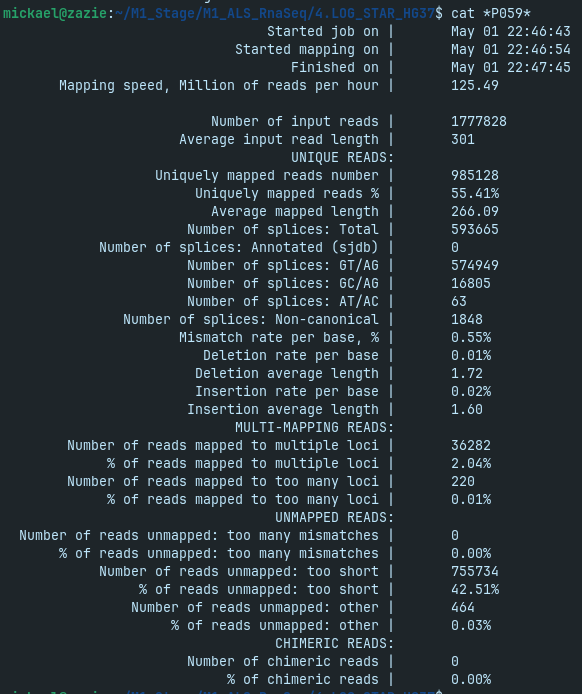
\includegraphics[width=\linewidth]{STAR_log.png}
    \caption*{log d'alignement avec STAR}
  \end{minipage}
  \hfill
  \begin{minipage}[b]{0.48\textwidth}
    \centering
    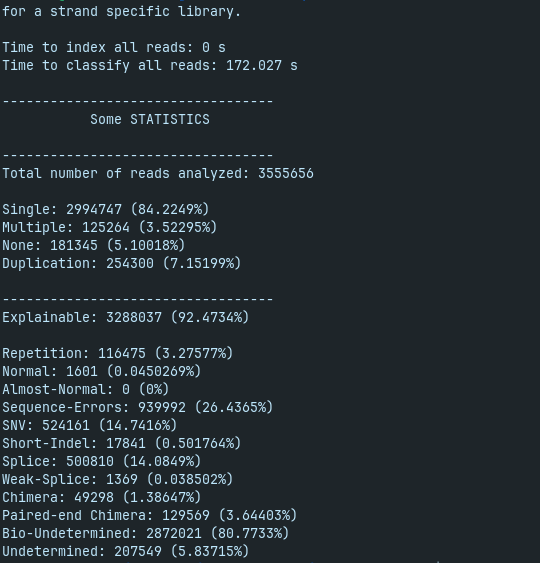
\includegraphics[width=\linewidth]{CRAC_summary.png}
    \caption*{summary généré par CRAC}
  \end{minipage}
  \caption{\underline{Comparaison visuelle des statistiques d’alignement STAR et CRAC.}}
  \label{fig:annexe_star_crac}	
\end{figure}
\newpage
\subsection{Modification du pipeline Snakemake}
\label{annexe:snake_ali}
   \centering
 \begin{lstlisting}[style=makefileStyle,caption={\underline{Règle Snakemake \texttt{aggregateStar} pour l'extraction des statistiques STAR}}]
rule aggregateStar:
    input:
        logs = expand(OUTPUT + "/STAR/results/{sample}/Log.final.out", sample=SAMPLES)
    output:
        csv = OUTPUT + "/STAR/Stats_Log_star.csv"
    shell:
    r"""
    # Headers generation :
    echo "Run,Patient,Type,STAR_Date_Mapping,STAR_Total_reads,\
    STAR_Unique_reads,STAR_Unique_pct,\
    STAR_Multi_reads,STAR_Multi_pct,\
    STAR_No_map_reads,STAR_No_map_pct_sum,STAR_No_map_pct_mismatch,\
    STAR_No_map_pct_tooshort,\
    STAR_No_map_pct_other,\
    STAR_Avg_read_len" > {output.csv}

    # Metrics extraction
    for logfile in {input.logs}; do
        basename=$(basename "$logfile")
        sample=$(echo "$basename" | sed -E 's/.+\/?([^\/]+)_Log.final.out/\1/')
        Run=$(echo "$sample" | cut -d '-' -f1)
        Patient=$(echo "$sample" | cut -d '-' -f2)
        Type=$(echo "$sample" | cut -d '-' -f3 | cut -d '.' -f1)

        Ext() {
            grep "$1" "$logfile" | cut -d '|' -f2 | tr -d ' ' | tr -d '%' || echo "0"
        }
        STAR_Date_Mapping=$(Ext "Finished on")
        STAR_Total_reads=$(Ext "Number of input reads")
        STAR_Unique_reads=$(Ext "Uniquely mapped reads number")
        STAR_Unique_pct=$(Ext "Uniquely mapped reads %")
        ...
        echo "$Run,$Patient,$Type,$STAR_Date_Mapping,$STAR_Total_reads,\
        $STAR_Unique_reads,$STAR_Unique_pct,\
        $STAR_Multi_reads,$STAR_Multi_pct,\
        $STAR_No_map_reads,$STAR_No_map_pct_sum,$STAR_No_map_pct_mismatch,\
        $STAR_No_map_pct_tooshort,$STAR_No_map_pct_other,\
        $STAR_Avg_read_len" >> {output.csv}
    done
    """
\end{lstlisting}



\printglossary[title=Glossaire]

\newpage
\section{Bibliographie compilée}
\renewcommand{\bibname}{Bibliographie compilée}
\printbibliography[heading=none]  

\end{document}
